% -*- latex -*-
%%%%%%%%%%%%%%%%%%%%%%%%%%%%%%%%%%%%%%%%%%%%%%%%%%%%%%%%%%%%%%%%
%%%%%%%%%%%%%%%%%%%%%%%%%%%%%%%%%%%%%%%%%%%%%%%%%%%%%%%%%%%%%%%%
%%%%
%%%% This text file is part of the source of 
%%%% `Parallel Programming in MPI and OpenMP'
%%%% by Victor Eijkhout, copyright 2012-6
%%%%
%%%% omp-loop.tex : the OpenMP loop construct
%%%%
%%%%%%%%%%%%%%%%%%%%%%%%%%%%%%%%%%%%%%%%%%%%%%%%%%%%%%%%%%%%%%%%
%%%%%%%%%%%%%%%%%%%%%%%%%%%%%%%%%%%%%%%%%%%%%%%%%%%%%%%%%%%%%%%%

\Level 0 {Loop parallelism}
\label{sec:omp-for}

Loop parallelism is a very common type of parallelism in scientific
codes, so OpenMP has an easy mechanism for it.
OpenMP parallel loops are a first example of OpenMP `worksharing'
constructs (see section~\ref{sec:work-sharing} for the full list):
constructs that take an amount of work and distribute it over the
available threads in a parallel region.

The parallel execution of a loop can be handled a number of different ways.
For instance, you can create a parallel region around the loop, and
adjust the loop bounds:
\begin{verbatim}
#pragma omp parallel
{
  int threadnum = omp_get_thread_num(),
    numthreads = omp_get_num_threads();
  int low = N*threadnum/numthreads,
    high = N*(threadnum+1)/numthreads;
  for (i=low; i<high; i++)
    // do something with i
}
\end{verbatim}

A more natural option is to use the
\indexpragma{parallel for} pragma:
\begin{verbatim}
#pragma omp parallel
#pragma omp for
for (i=0; i<N; i++) {
  // do something with i
}
\end{verbatim}
This has several advantages. For one, you don't have to calculate the loop bounds
for the threads yourself, but you can also tell OpenMP to assign the loop
iterations according to different schedules (section~\ref{sec:schedule}).

Figure~\ref{fig:omp-par-do} shows the execution on four threads of
\begin{verbatim}
#pragma omp parallel
{
  code1();
#pragma omp for
  for (i=1; i<=4*N; i++) {
    code2();
  }
  code3();
}
\end{verbatim}
The code before and after the loop is executed identically
in each thread; the loop iterations are spread over the four threads.
\begin{figure}[ht]
  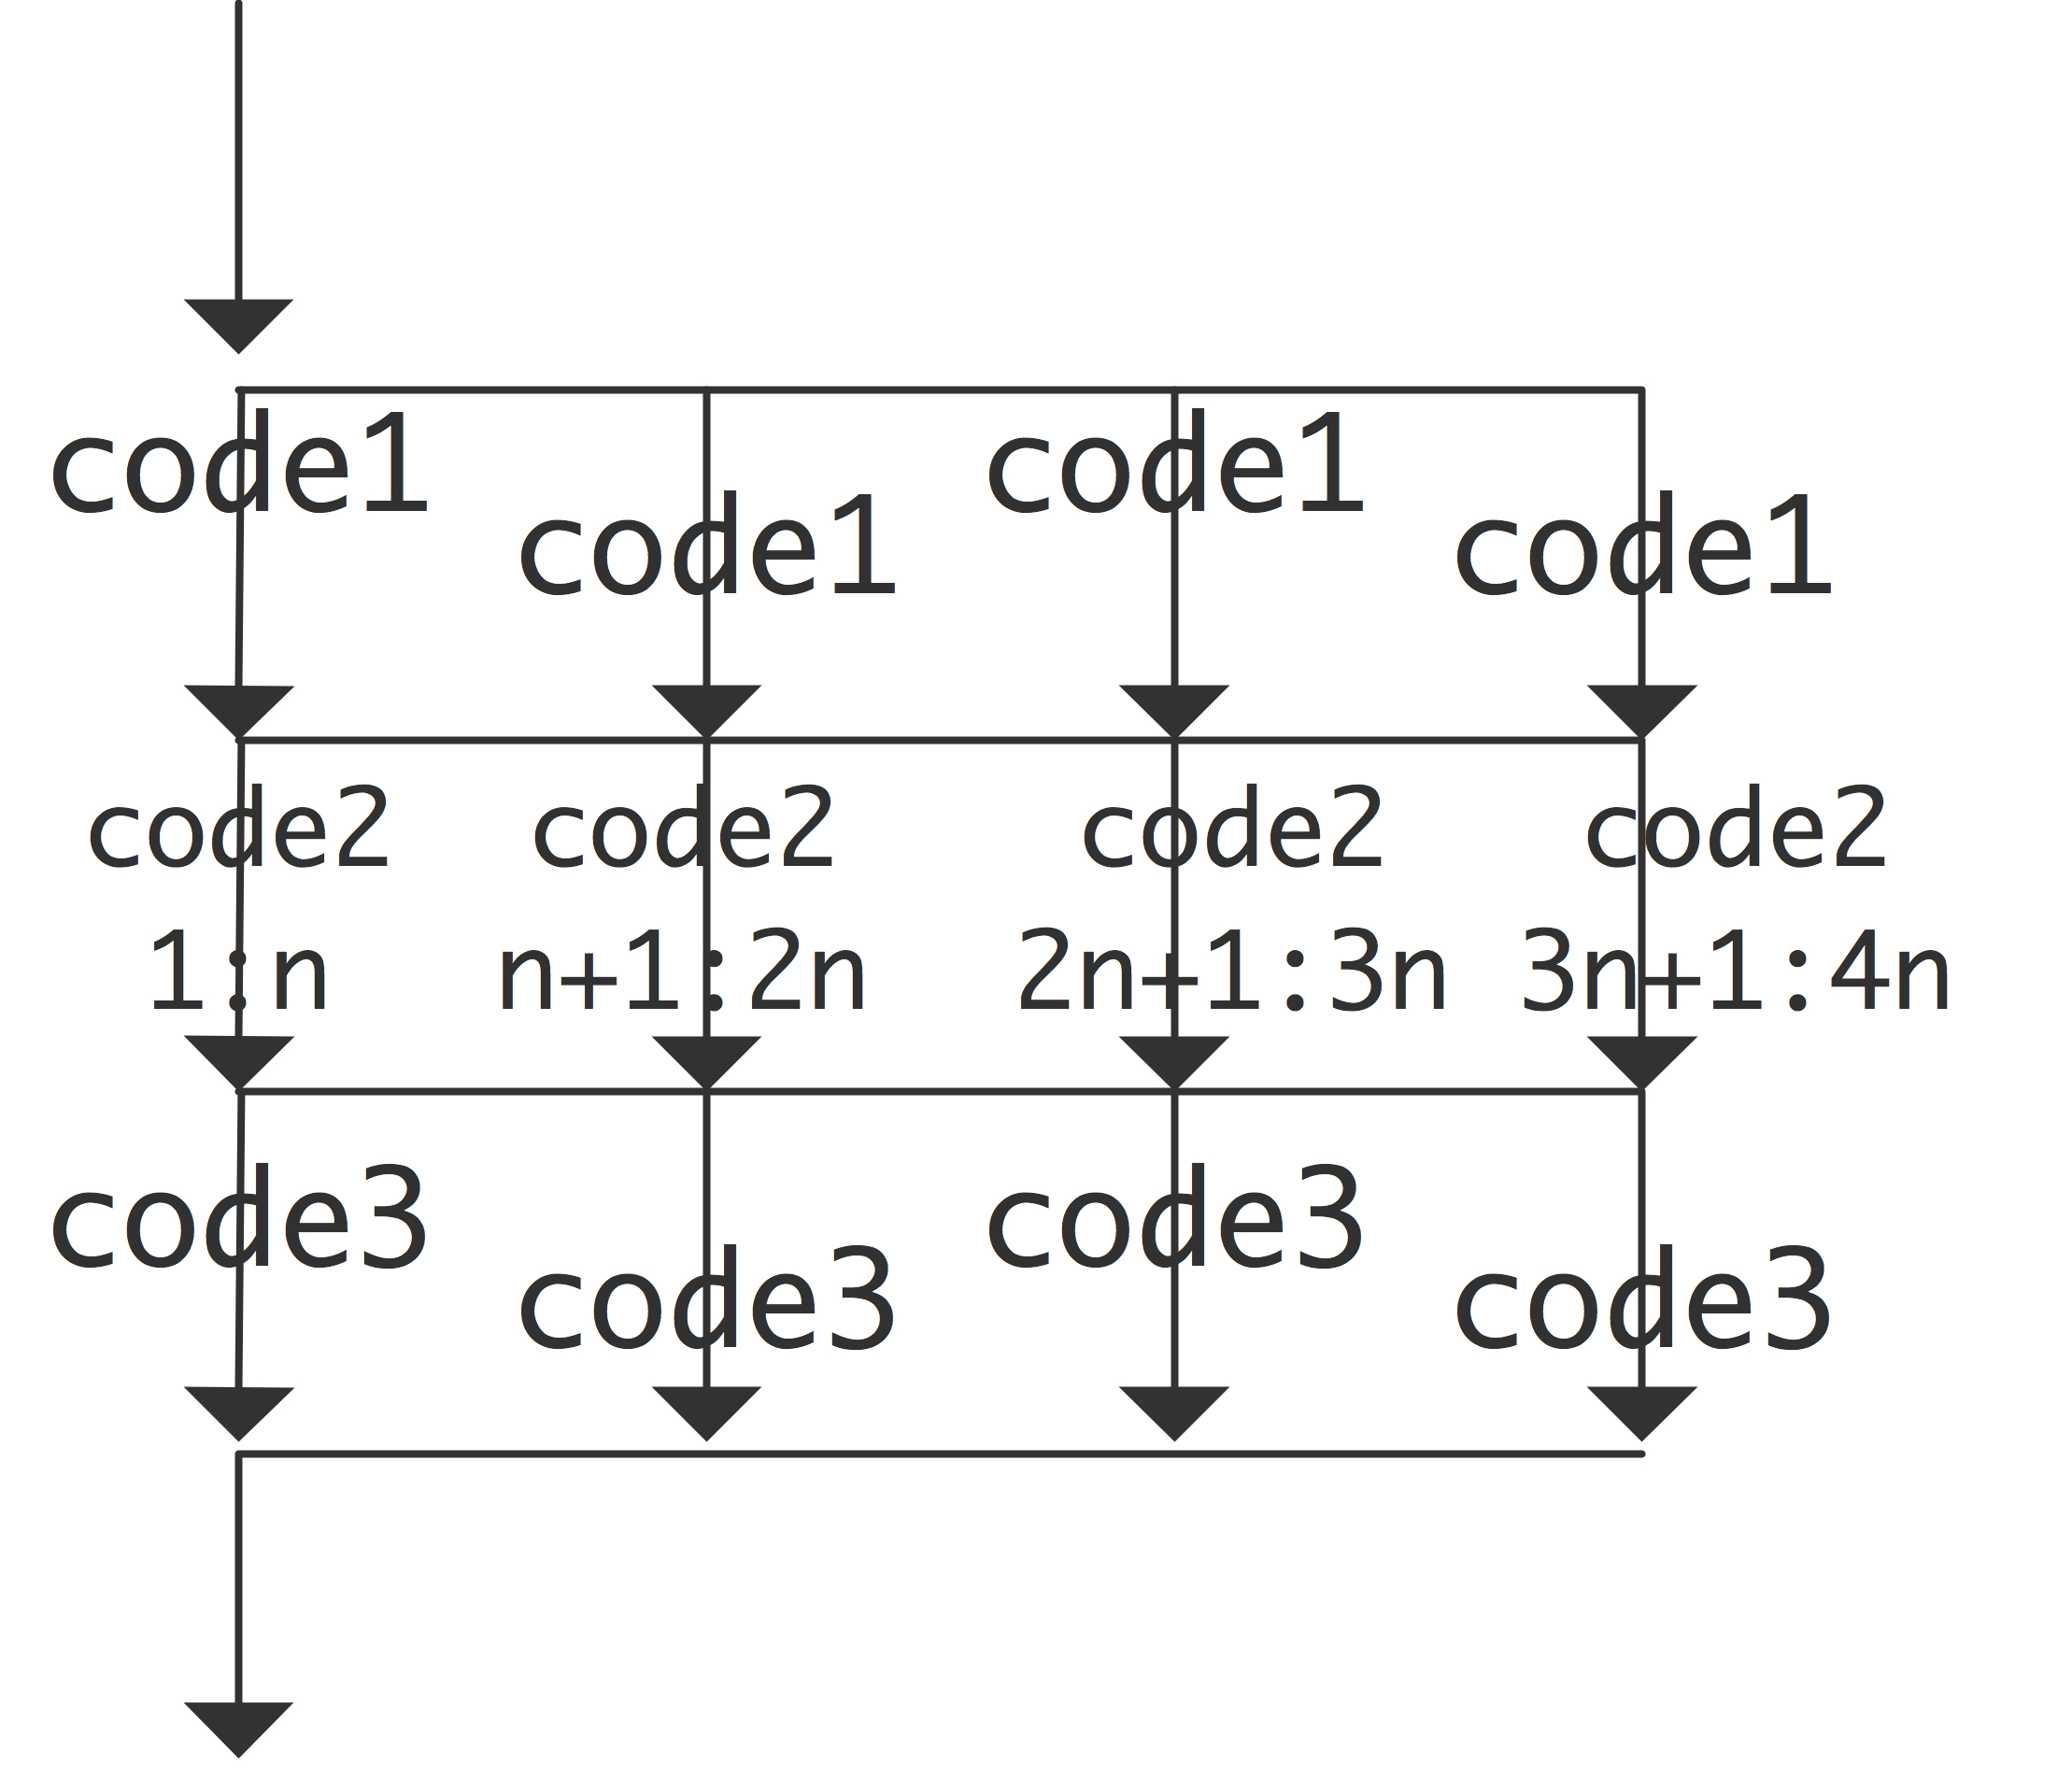
\includegraphics[scale=.1]{parallel-do}
  \caption{Execution of parallel code inside and outside a loop}
  \label{fig:omp-par-do}
\end{figure}

Note that the \n{parallel do} and \n{parallel for}
pragmas do not create a team of threads: they
take the team of threads that is active,
and divide the loop iterations over them.

This means that the \n{omp for} or \n{omp do} directive needs to be
inside a parallel region. It is also possible to have a combined
\n{omp parallel for} or \n{omp parallel do} directive.

If your parallel region only contains a loop, you can combine the
pragmas for the parallel region and distribution of the loop iterations:
\begin{verbatim}
#pragma omp parallel for
  for (i=0; .....
\end{verbatim}

\begin{exercise}
  \label{ex:omp-pi}
  Compute $\pi$ by \indexterm{numerical integration}. We use the fact that $\pi$
  is the area of the unit circle, and we approximate this by computing
  the area of a quarter circle using \indexterm{Riemann sums}.
  \begin{itemize}
  \item Let $f(x)=\sqrt{1-x^2}$ be the function that describes the
    quarter circle for $x=0\ldots 1$;
  \item Then we compute \[ \pi/4\approx\sum_{i=0}^{N-1} \Delta x
    f(x_i) \qquad \hbox{where $x_i=i\Delta x$ and $\Delta x=1/N$} \]
  \end{itemize}
  Write a program for this, and parallelize it using OpenMP parallel
  for directives.
  \begin{enumerate}
  \item Put a \n{parallel} directive around your loop. Does it still
    compute the right result? Does the time go down with the number of
    threads? (The answers should be no and no.)
  \item Change the \n{parallel} to \n{parallel for} (or \n{parallel
    do}). Now is the result correct? Does execution speed up? (The
    answers should now be no and yes.)
  \item Put a \n{critical} directive in front of the update. (Yes and
    very much no.)
  \item Remove the \n{critical} and add a clause
    \n{reduction(+:quarterpi)} to the \n{for} directive.
    Now it should be correct and efficient.
  \end{enumerate}
  Use different numbers of cores and compute the
  speedup you attain over the sequential computation. Is there a
  performance difference between the OpenMP code with 1~thread and the
  sequential code?
\end{exercise}

\begin{remark}
  In this exercise you may have seen the runtime go up a couple of times
  where you weren't expecting it. The issue here is \indexterm{false
    sharing}; see~\HPSCref{sec:roundoff-parallel} for more explanation.
\end{remark}

There are some restrictions on the loop: basically, OpenMP needs to be
able to determine in advance how many iterations there will be.
\begin{itemize}
\item The loop can not contains \n{break}, \n{return}, \n{exit} statements, or
  \n{goto} to a label outside the loop.
\item The \n{continue} (C) or \n{cycle} (F) statement is allowed.
\item The index update has to be an increment (or decrement) by a fixed amount.
\item The loop index variable is automatically private, and not changes to it
  inside the loop are allowed.
\end{itemize}

\Level 0 {Loop schedules}
\label{sec:schedule}

Usually you will have many more iterations in a loop than there are threads.
Thus, there are several ways you can assign your loop iterations to the threads.
OpenMP lets you specify this with the \indextermtt{schedule} clause.
\begin{verbatim}
#pragma omp for schedule(....)
\end{verbatim}

The first distinction we now have to make is between static and dynamic schedules.
With static schedules, the iterations are assigned purely based on the number
of iterations and the number of threads (and the \n{chunk} parameter; see later).
In dynamic schedules, on the other hand, iterations are assigned to threads that
are unoccupied. Dynamic schedules are a good idea if iterations take an unpredictable
amount of time, so that \indexterm{load balancing} is needed.

\begin{figure}[ht]
  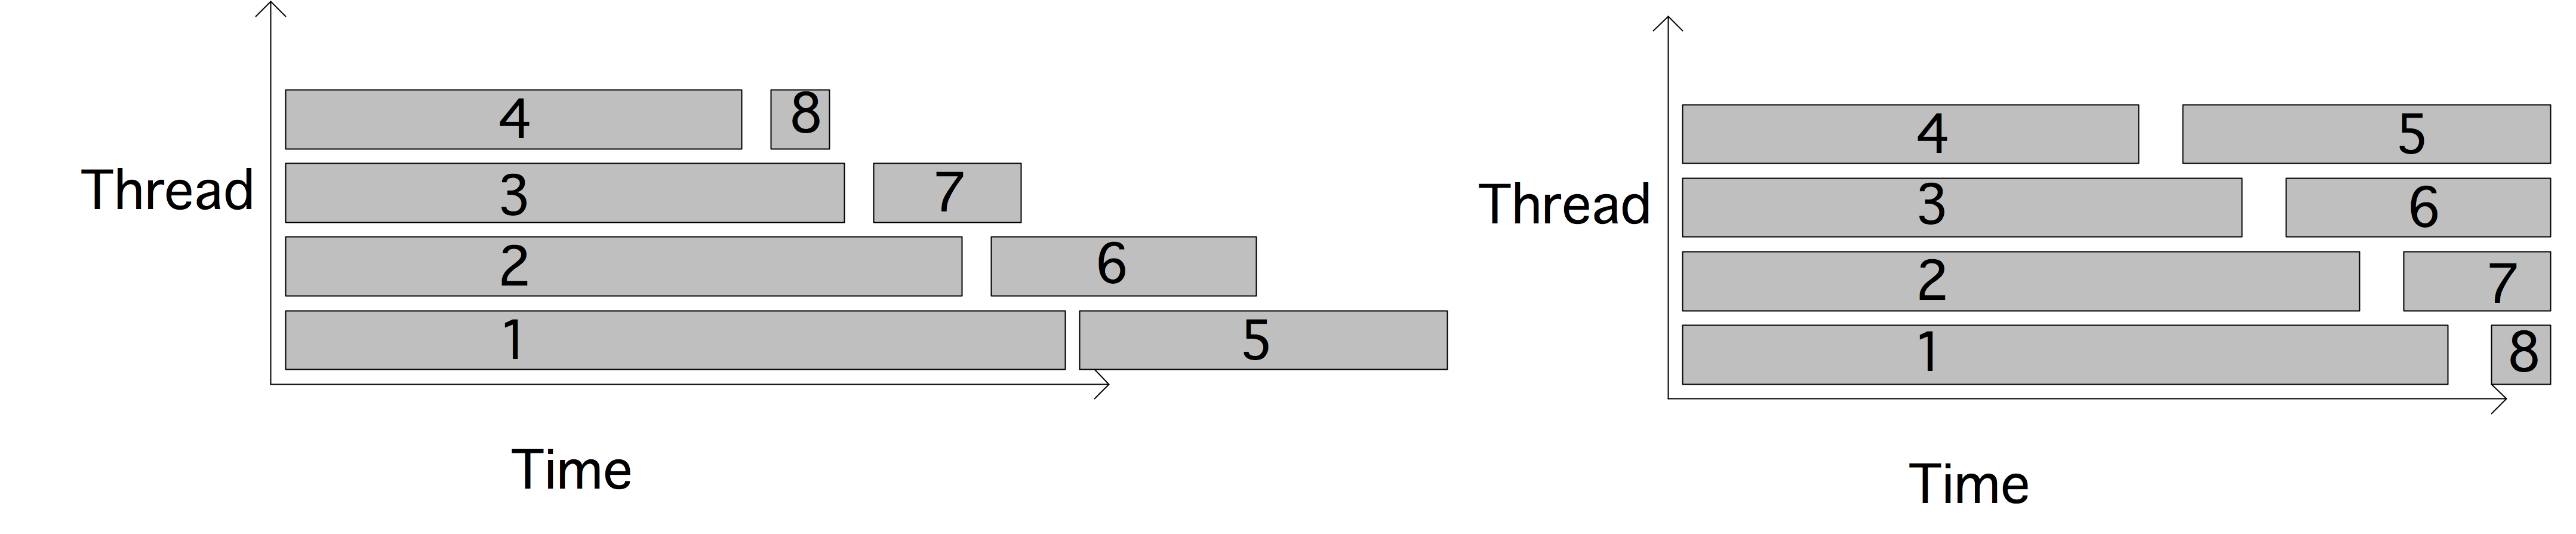
\includegraphics[scale=.07]{scheduling}
  \caption{Illustration static round-robin scheduling versus dynamic}
  \label{fig:omp-robin}
\end{figure}
%
Figure~\ref{fig:omp-robin} illustrates this: assume that each core
gets assigned two (blocks of) iterations and these blocks take
gradually less and less time. You see from the left picture that
thread~1 gets two fairly long blocks, where as thread~4 gets two short
blocks, thus finishing much earlier. (This phenomenon of threads
having unequal amounts of work is known as \indexterm{load
  imbalance}.) On the other hand, in the right figure thread~4 gets
block~5, since it finishes the first set of blocks early. The effect
is a perfect load balancing.

\begin{figure}[ht]
  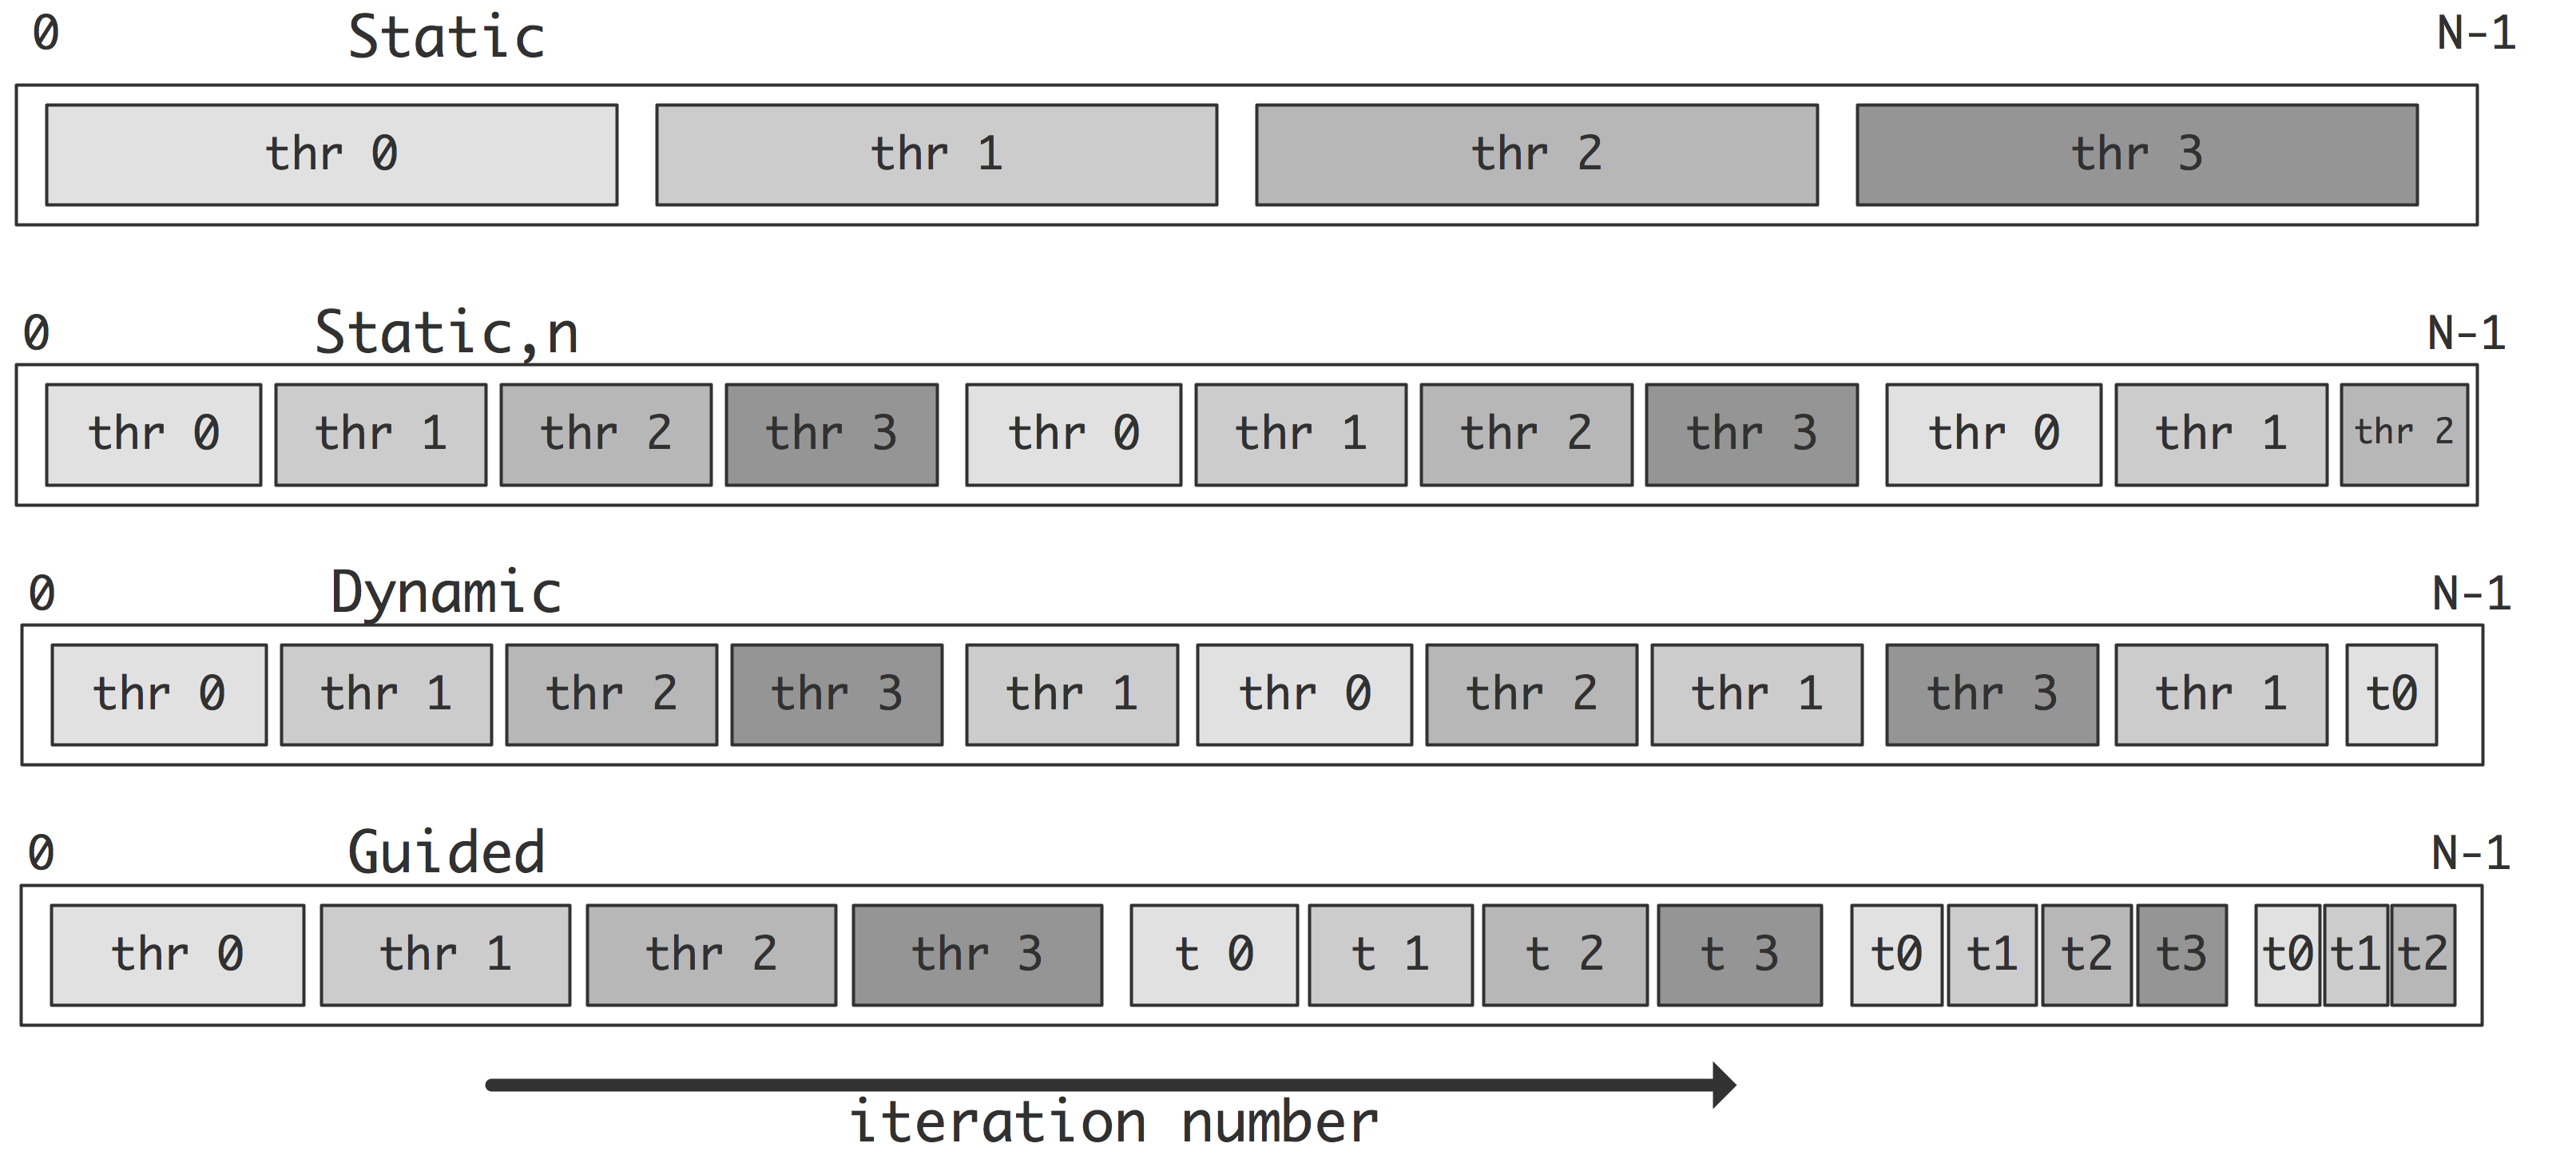
\includegraphics[scale=.12]{schedules}
  \caption{Illustration of the scheduling strategies of loop iterations}
  \label{fig:omp-schedule}
\end{figure}

The default static schedule is to assign one consecutive block of
iterations to each thread. If you want different sized blocks you can
defined a \indexclauseoption{schedule}{chunk} size:
\begin{verbatim}
#pragma omp for schedule(static[,chunk])
\end{verbatim}
(where the square brackets indicate an optional argument).
With static scheduling, the compiler will split up the loop iterations at compile time,
so, provided the iterations take roughly the same amount of time, this is the most efficient at runtime.

The choice of a chunk size is often a balance between the low overhead of having 
only a few chunks, versus the load balancing effect of having smaller chunks.
\begin{exercise}
  Why is a chunk size of~1 typically a bad idea? (Hint: think about
  cache lines, and read \HPSCref{sec:falseshare}.)
\end{exercise}

In dynamic scheduling OpenMP will put blocks of iterations
(the default chunk size is~1) in a task queue, and the threads take one of these
tasks whenever they are finished with the previous.
\begin{verbatim}
#pragma omp for schedule(static[,chunk])
\end{verbatim}
While this schedule may give good load balancing if the iterations
take very differing amounts of time to execute, it does carry runtime
overhead for managing the queue of iteration tasks.

Finally, there is the \indexclauseoption{schedule}{guided} schedule, which gradually decreases the chunk size.
The thinking here is that large chunks carry the least overhead, but smaller chunks are better
for load balancing.
%
The various schedules are illustrated in figure~\ref{fig:omp-schedule}.

If you don't want to decide on a schedule in your code, you can
specify the \indexclauseoption{schedule}{runtime} schedule. The actual
schedule will then at runtime be read from the
\indextermtt{OMP_SCHEDULE} environment variable. You can even just
leave it to the runtime library by specifying
\indexclauseoption{schedule}{auto}

\begin{exercise}
  \label{ex:omp-pi-adapt}
  %
  We continue with exercise~\ref{ex:omp-pi}.  We add `adaptive
  integration': where needed, the program refines the step
  size\footnote{It doesn't actually do this in a mathematically
    sophisticated way, so this code is more for the sake of the
    example.}.  This means that the iterations no longer take a
  predictable amount of time.

\begin{minipage}{.3\linewidth}\small
\begin{verbatim}
for (i=0; i<nsteps; i++) {
 double
   x = i*h,x2 = (i+1)*h,
   y = sqrt(1-x*x),y2 = sqrt(1-x2*x2),
   slope = (y-y2)/h;
 if (slope>15) slope = 15;
 int
   samples = 1+(int)slope, is;
 for (is=0; is<samples; is++) {
   double
     hs = h/samples,
     xs = x+ is*hs,
     ys = sqrt(1-xs*xs);
   quarterpi += hs*ys;
   nsamples++;
 }
}
pi = 4*quarterpi;
\end{verbatim}
\end{minipage}

\begin{enumerate}
\item Use the \n{omp parallel for} construct to parallelize the loop.
  As in the previous lab, you may at first see an incorrect result.
  Use the \n{reduction} clause to fix this.
\item Your code should now see a decent speedup, using up to 8~cores.
  However, it is possible to get completely linear speedup. For this
  you need to adjust the schedule.

  Start by using \n{schedule(static,$n$)}. Experiment with values
  for~$n$.  When can you get a better speedup? Explain this.
\item Since this code is somewhat dynamic, try \n{schedule(dynamic)}.
  This will actually give a fairly bad result. Why?  Use
  \n{schedule(dynamic,$n$)} instead, and experiment with values
  for~$n$.
\item Finally, use \n{schedule(guided)}, where OpenMP uses a
  heuristic.  What results does that give?
\end{enumerate}
     
\end{exercise}

\begin{exercise}
  Program the \indexterm{LU factorization} algorithm without pivoting.
\begin{verbatim}
for k=1,n:
  A[k,k] = 1./A[k,k]
  for i=k+1,n:
    A[i,k] = A[i,k]/A[k,k]
    for j=k+1,n:
      A[i,j] = A[i,j] - A[i,k]*A[k,j]
\end{verbatim}
\begin{enumerate}
\item Argue that it is not possible to parallelize the outer loop.
\item Argue that it is possible to parallelize both the $i$ and $j$ loops.
\item Parallelize the algorithm by focusing on the $i$ loop. Why is the algorithm as given here best
  for a matrix on row-storage? What would you do if the matrix was on column storage?
\item Argue that with the default schedule, if a row is updated by one thread in one iteration,
  it may very well be updated by another thread in another. Can you find a way to schedule
  loop iterations so that this does not happen? What practical reason is there for doing so?
\end{enumerate}
\end{exercise}

The schedule can be declared explicitly, set at runtime
through the \indextermtt{OMP_SCHEDULE} environment variable, or left up to the runtime system
by specifying \n{auto}. Especially in the last two cases  you may want to enquire
what schedule is currently being used with
\indextermtt{omp_get_schedule}.
\begin{verbatim}
int omp_get_schedule(omp_sched_t * kind, int * modifier );
\end{verbatim}

Its mirror call is \indextermtt{omp_set_schedule}, which sets the
value that is used when schedule value \n{runtime} is used. It is in
effect equivalent to setting the environment variable
\n{OMP_SCHEDULE}.
\begin{verbatim}
void omp_set_schedule (omp_sched_t kind, int modifier);
\end{verbatim}

\begin{tabular}{|l|lll|}
  \hline
  Type&environment variable&clause&modifier default\\
        &{\tt OMP\_SCHEDULE\char`\=}&{\tt schedule( ... )}& \\
  \hline
  static&{static[,n]}&{static[,n]}&$N/\mathit{nthreads}$\\
  dynamic&{dynamic[,n]}&{dynamic[,n]}&$1$\\
  guided&{guided[,n]}&{guided[,n]}\\
  \hline
\end{tabular}

Here are the various schedules you can set with the
\n{schedule}\index{schedule!clause} clause:
\begin{description}
  \item[affinity] Set by using value  \indextermtt{omp_sched_affinity}
  \item[auto] The schedule is left up to the implementation. Set by
    using value \indextermtt{omp_sched_auto}
  \item[dynamic] value:~2. The modifier parameter is the
    \indexterm{chunk} size; default~1. Set by using value
    \indextermtt{omp_sched_dynamic}
  \item[guided] Value:~3. The modifier parameter is the
    \indextermtt{chunk} size. Set by using value
    \indextermtt{omp_sched_guided}
  \item[runtime] Use the value of the \indextermtt{OMP_SCHEDULE}
    environment variable. Set by using value
    \indextermtt{omp_sched_runtime}
  \item[static] value:~1. The modifier parameter is the \indexterm{chunk} size. Set by using value  \indextermtt{omp_sched_static}
\end{description}

\Level 0 {Reductions}

So far we have focused on loops with independent iterations.
Reductions are a common type of loop with dependencies.
There is an extended discussion of reductions in section~\ref{sec:reduction}.

\Level 0 {Collapsing nested loops}

In general, the more work there is to divide over a number of threads,
the more efficient the parallelization will be. In the context of
parallel loops, it is possible to increase the amount of work by
parallelizing all levels of loops instead of just the outer one.

Example: in
\begin{verbatim}
for ( i=0; i<N; i++ )
  for ( j=0; j<N; j++ )
    A[i][j] = B[i][j] + C[i][j] 
\end{verbatim}
all $N^2$ iterations are independent, but a regular \n{omp for}
directive will only parallelize one level. The \indexclause{collapse}
clause will parallelize more than one level:
\begin{verbatim}
#pragma omp for collapse(2)
for ( i=0; i<N; i++ )
  for ( j=0; j<N; j++ )
    A[i][j] = B[i][j] + C[i][j] 
\end{verbatim}
It is only possible to collapse perfectly nested loops, that is, the
loop body of the outer loop can consist only of the inner loop; there
can be no statements before or after the inner loop in the loop body
of the outer loop. That is, the two loops in
\begin{verbatim}
for (i=0; i<N; i++) {
  y[i] = 0.;
  for (j=0; j<N; j++)
    y[i] + A[i][j] * x[j]
  }
\end{verbatim}
can not be collapsed.

\begin{exercise}
  Can you rewrite the preceding code example so that it can be
  collapsed?
  Do timing tests to see if you can notice the improvement from collapsing.
\end{exercise}

\Level 0 {Ordered iterations}
\label{sec:omp-ordered}

Iterations in a parallel loop that are execution in parallel do not
execute in lockstep. That means that in
\begin{verbatim}
#pragma omp parallel for
for ( ... i ... ) {
  ... f(i) ...
  printf("something with %d\n",i);
}
\end{verbatim}
it is not true that all function evaluations happen more or less at
the same time, followed by all print statements. The print statements
can really happen in any order. The \indexclause{ordered} clause
coupled with the \indexpragma{ordered} directive can
force execution in the right order:
\begin{verbatim}
#pragma omp parallel for ordered
for ( ... i ... ) {
  ... f(i) ...
#pragma omp ordered
  printf("something with %d\n",i);
}
\end{verbatim}
Example code structure:
\begin{verbatim}
#pragma omp parallel for shared(y) ordered
for ( ... i ... ) {
  int x = f(i)
#pragma omp ordered
  y[i] += f(x)
  z[i] = g(y[i])
}
\end{verbatim}
There is a limitation:
each iteration can encounter only one \n{ordered} directive.

\Level 0 {\texttt{nowait}}
\label{sec:omp-nowait}

The implicit barrier at the end of a work sharing construct
can be cancelled with a \indexclause{nowait} clause.
This has the effect that threads that are finished can continue
with the next code in the parallel region:
\begin{verbatim}
#pragma omp parallel
{
#pragma omp for nowait
  for (i=0; i<N; i++) { ... }
  // more parallel code
}
\end{verbatim}

In the following example, threads that are finished with the first loop
can start on the second. Note that this requires both loops to have
the same schedule.
\begin{verbatim}
#pragma omp parallel
{
  x = local_computation()
#pragma omp for nowait
  for (i=0; i<N; i++) { 
    x[i] = ... 
  }
#pragma omp for 
  for (i=0; i<N; i++) { 
    y[i] = ... x[i] ...
  }
}
\end{verbatim}

\Level 0 {While loops}

OpenMP can only handle `for' loops: \indexterm{while loops} can not
be parallelized. So you have to find a way around that. While loops
are for instance used to search through data:
\begin{verbatim}
while ( a[i]!=0 && i<imax ) {
 i++; }
// now i is the first index for which \n{a[i]} is zero.
\end{verbatim}
We replace the while loop by a for loop that examines all locations:
\begin{verbatim}
result = -1;
#pragma omp parallel for
for (i=0; i<imax; i++) {
  if (a[i]!=0 && result<0) result = i;
}
\end{verbatim}
\begin{exercise}
  Show that this code has a race condition.
\end{exercise}
You can fix the race condition by making the condition into a critical section;
section~\ref{sec:critical}. In this particular example, with a very small amount
of work per iteration, that is likely to be inefficient 
in this case (why?).
A~more efficient solution uses the \indexpragma{lastprivate} pragma:
\begin{verbatim}
result = -1;
#pragma omp parallel for lastprivate(result)
for (i=0; i<imax; i++) {
  if (a[i]!=0) result = i;
}
\end{verbatim}
You have now solved a slightly different problem: the result variable
contains the \emph{last} location where \n{a[i]} is zero.

